\section{Gestion des tournois}

\textbf{Si vous êtes un membre du staff, et que vous avez la permission de gérer les tournois}, vous pouvez alors accéder à la page de gestion des tournois, depuis l'onglet \enquote{Staff} tout à droite du menu de navigation.

\begin{figure}[H]
\centering
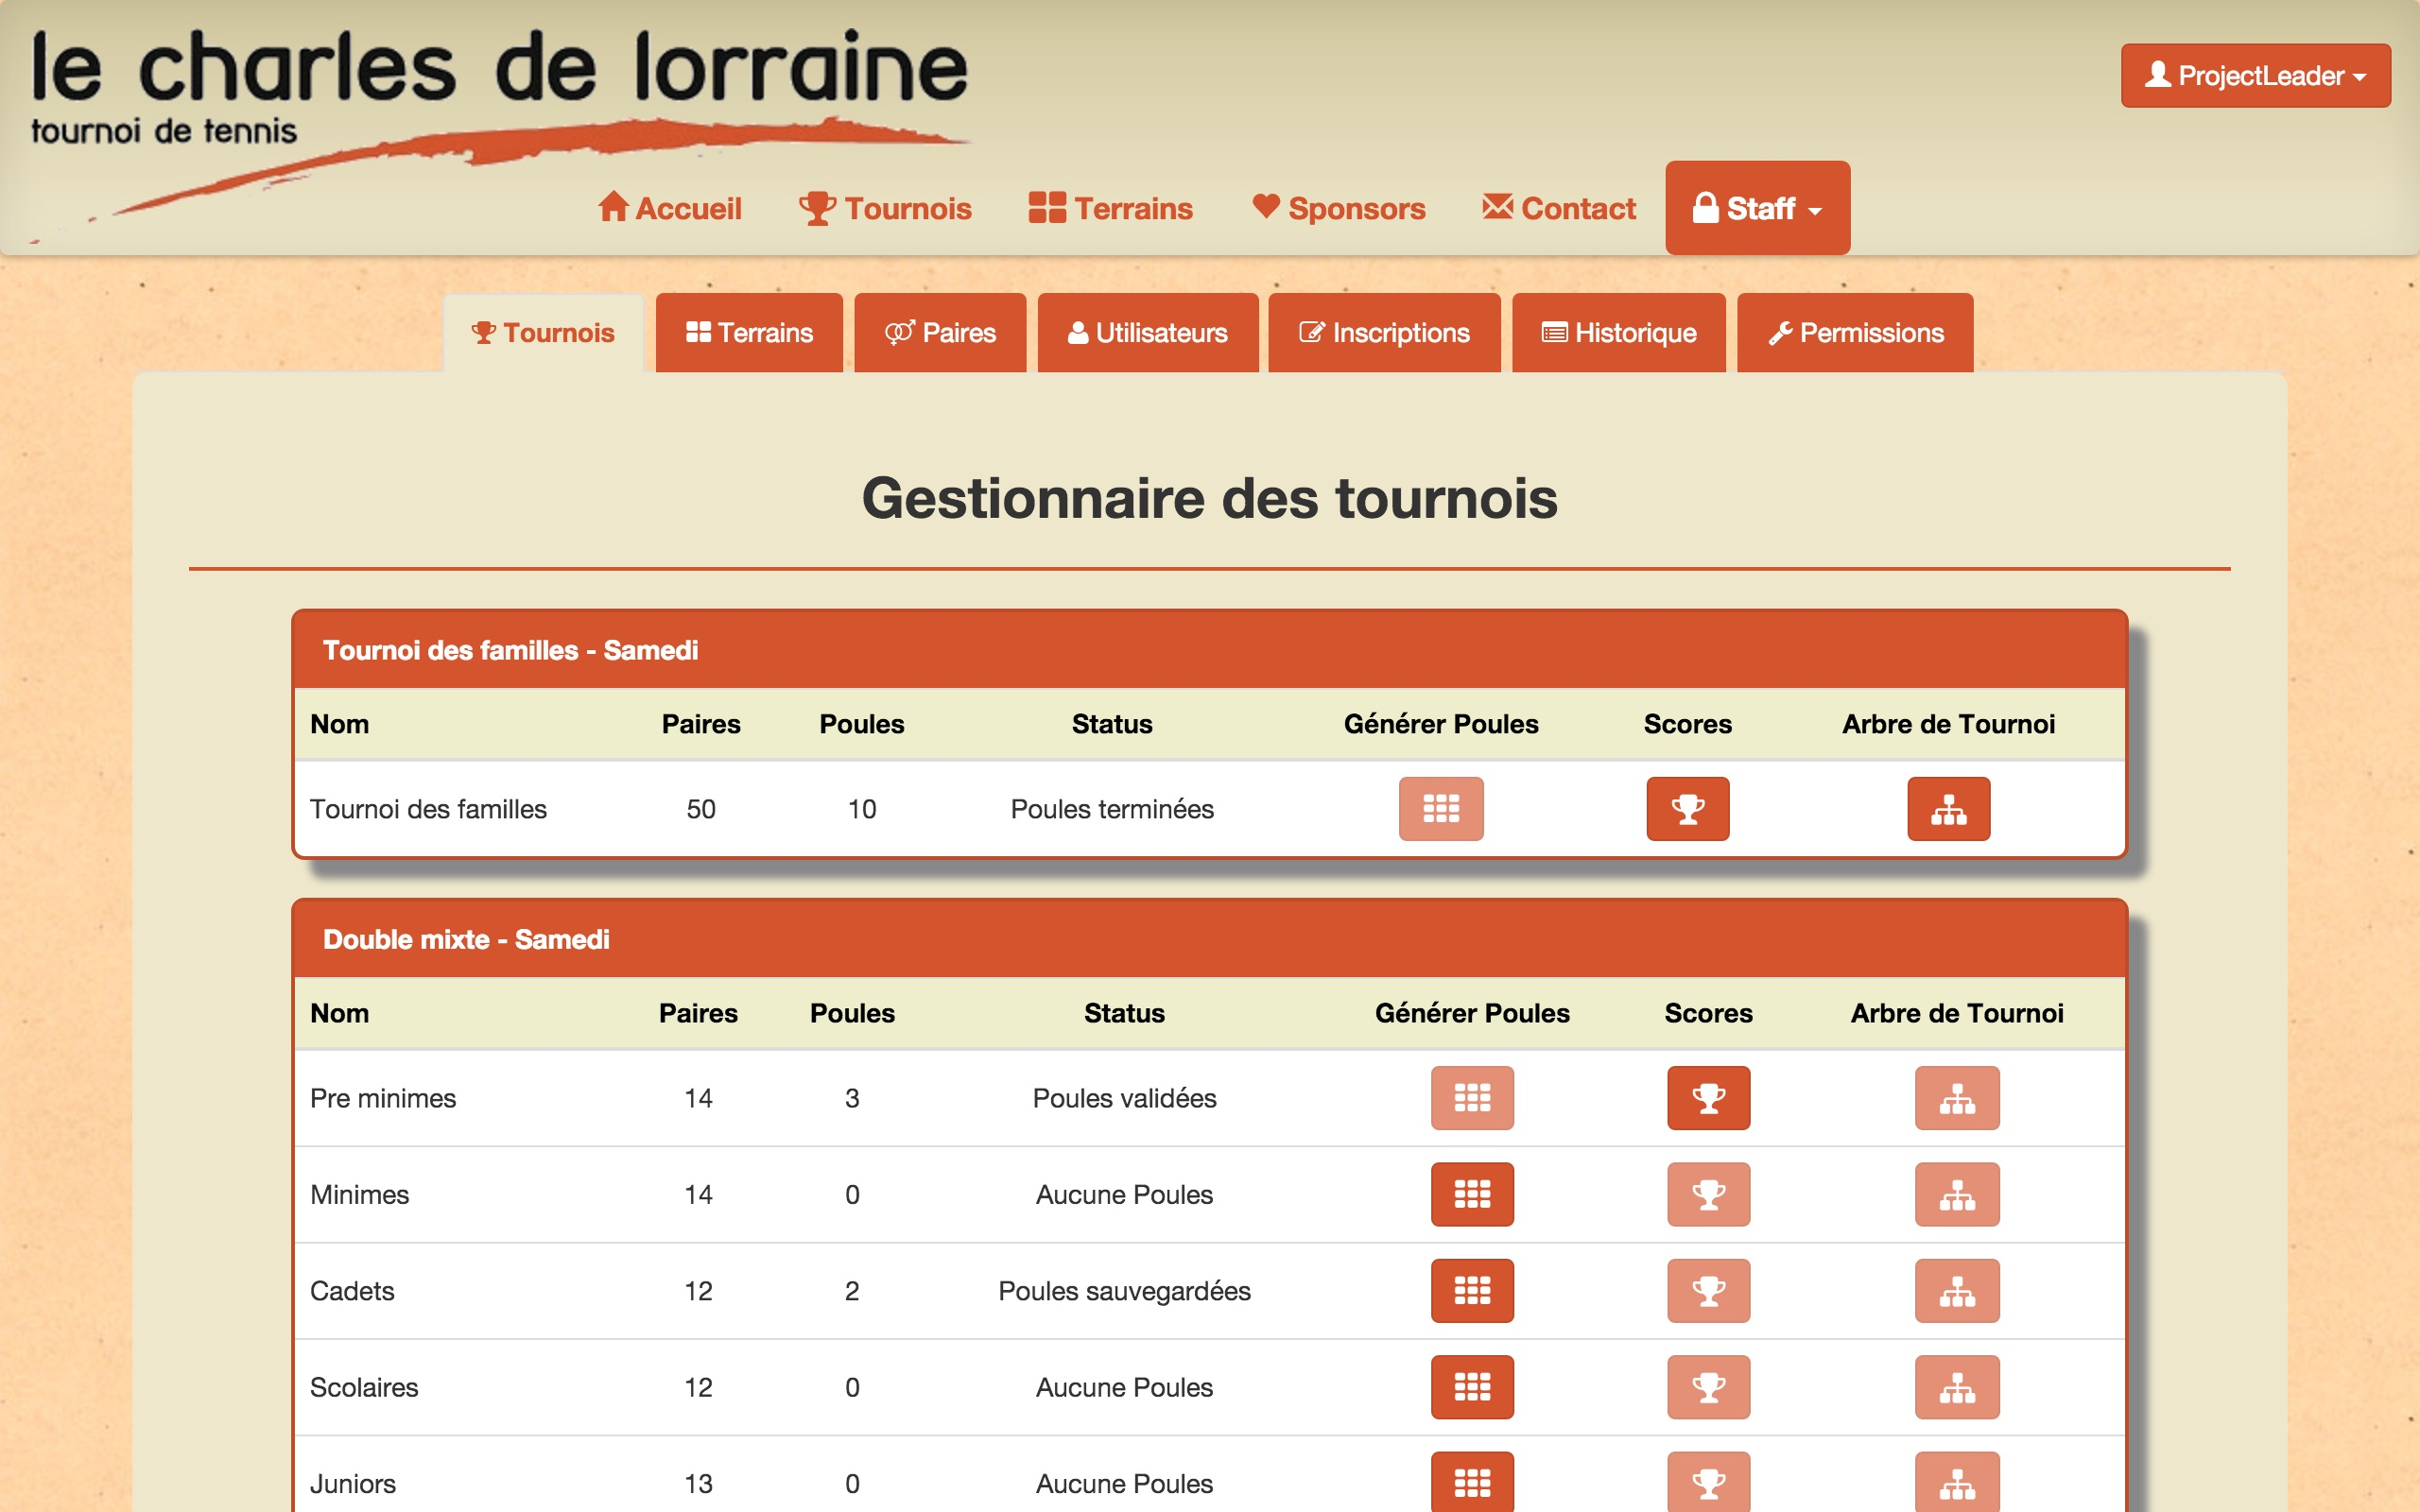
\includegraphics[scale=0.15]{gestion-tournois/gestion-tournois.jpg}
\caption{Page de la gestion des tournois}
\end{figure}

\subsection{Les tournois}

Depuis la page staff \enquote{Gestionnaire des tournois}, vous pouvez gérer tous les tournois et catégories dont vous avez eu préalablement la permission de gérer. Pour donner la permission à un utilisateur de gérer certains tournois, l'admin doit lui octroyer les permission à partir de la page \enquote{Gestionnaire des permissions} \ref{Gestion des permissions}.\newline =

Sur cette page, vous pouvez consulter une liste de tournois. Les tournois sont catégorisés en fonction du type du tournoi :

\begin{itemize}
\item \textit{Tournoi des familles}
\item \textit{Double mixte}
\item \textit{Double hommes}
\item \textit{Double femmes}
\end{itemize}

\begin{figure}[H]
\centering
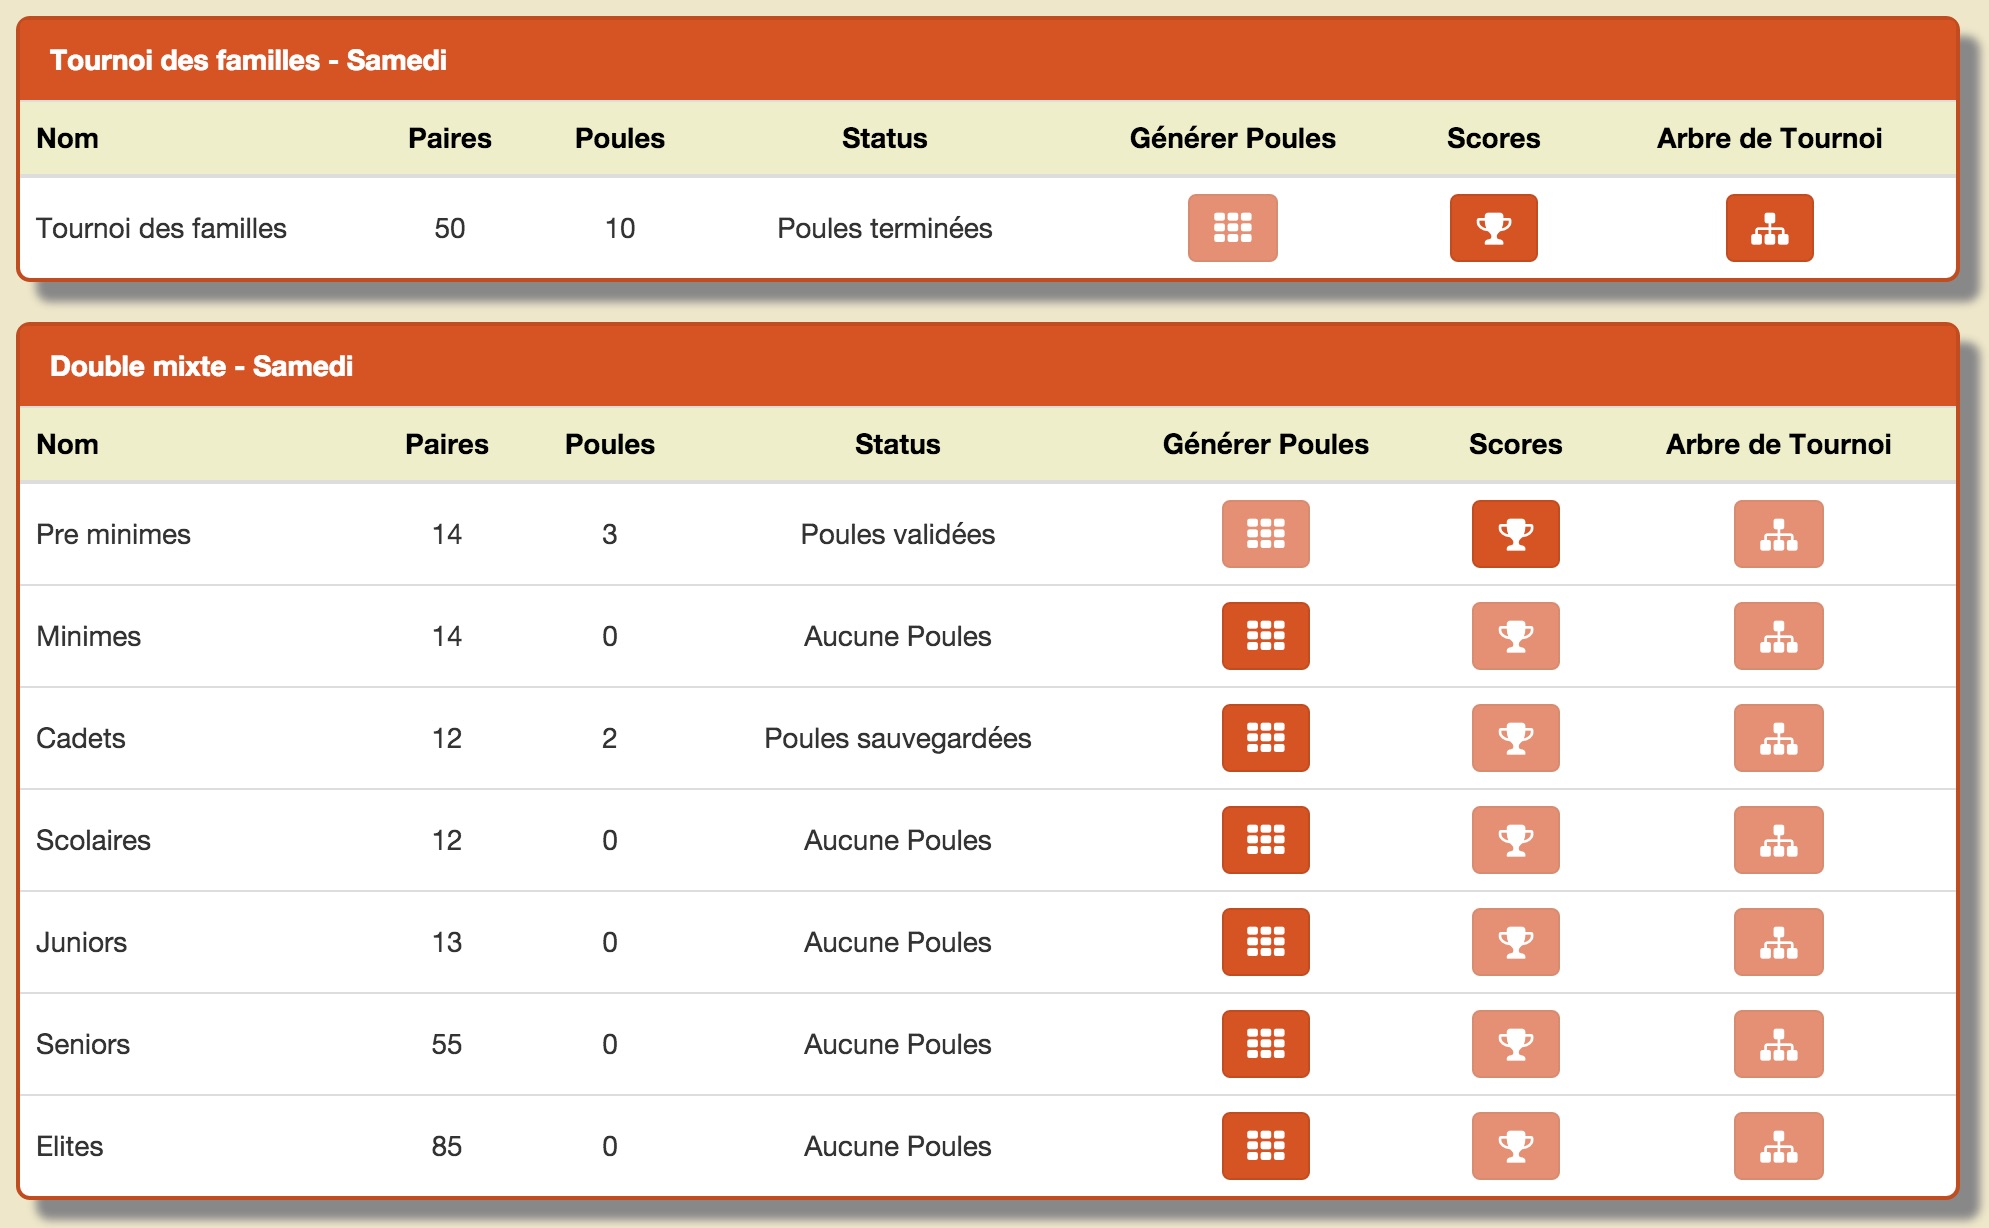
\includegraphics[scale=0.17]{gestion-tournois/gestion-tournois-liste.jpg}
\caption{Page de la gestion des tournois - liste des tournois}
\end{figure}

Tous les tournois, sauf le \textit{Tournoi des familles}, sont à nouveau catégorisés en fonction de l'âge des joueurs. Ces sous-tournois sont ordonnés du tournoi des plus jeunes, \textit{Pré-minimes}, au plus âgés, \textit{Élites}.\newline

Chaque tournois indique les informations les plus importantes, à savoir :

\begin{itemize}
\item \textit{le nombre de paires inscrites} ;
\item \textit{le nombre de poules actuel} ;
\item \textit{le status du tournoi}
\end{itemize}
\bigskip

Le status du tournoi impose les opérations possibles sur le tournoi. Par exemple :

\begin{itemize}
\item  \textbf{Aucune poules} n'autorise que de générer les poules ;
\item \textbf{Poules validées} permet d'encoder les scores ;
\item \textbf{Poules terminées} permet de consulter les poules, et de créer l'arbre d'élimination.
\end{itemize}
\bigskip

Il y a 3 boutons d'accès aux pages spécifiques de gestion des tournois, selon le status de celui-ci :

\begin{itemize}
\item \textit{Générer Poules} : permet de créer, modifier, et sauvegarder les poules ;
\item \textit{Scores} : permet de consulter les poules créées, supprimer les poules, imprimer les \textit{score boards}, et encoder les scores de chaque poule ;
\item \textit{Arbre de Tournoi} : permet de créer l'arbre du tournoi, imprimer l'arbre, et encoder les scores dans l'arbre
\end{itemize}

\begin{figure}[H]
\centering
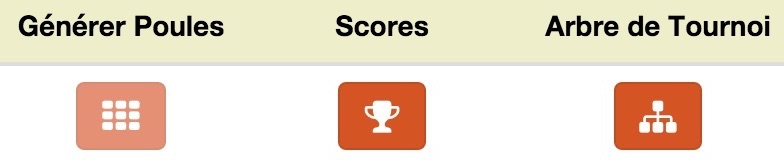
\includegraphics[scale=0.35]{gestion-tournois/gestion-tournois-operations.jpg}
\caption{Page de la gestion des tournois - accès aux pages spécifiques de gestion}
\end{figure}

\subsection{Les poules}

Toutes les fonctionnalités des tournois propres aux poules dépendent du status du tournoi, comme décrit à la section sur la liste des tournois.\newline

Il existe deux pages pour interagir avec les poules d'un tournoi :

\begin{itemize}
\item \textbf{Création des poules}, à partir du bouton \textit{Générer Poules} ;
\item \textbf{Gestion des poules}, à partir du bouton \textit{Scores}
\end{itemize}

\subsubsection{Création des poules}

La première page des poules d'un tournoi est la création des poules. Elle est accessible à partir de la page \enquote{Gestionnaire des tournois}, en cliquant sur le bouton du tournoi qui se trouve à la colonne \textit{Générer Poules}.

\begin{figure}[H]
\centering
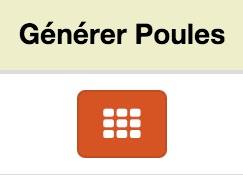
\includegraphics[scale=0.35]{creation-poules/creation-poules-bouton.jpg}
\caption{Bouton d'accès à la page de création des poules}
\end{figure}

Ce bouton est cliquable uniquement lorsque le status du tournoi est :

\begin{itemize}
\item \textbf{Aucune poules} : c'est le status initial d'un tournoi ;
\item \textbf{Poules sauvegardées} : c'est le status du tournoi lorsque les poules sont en cours de création, mais qu'elles n'ont pas encore totalement validées.
\end{itemize}
\bigskip

La page de création de poules se présente avec un module de configuration de toutes les poules, et plusieurs modules correspondant aux poules du tournoi.

\begin{figure}[H]
\centering
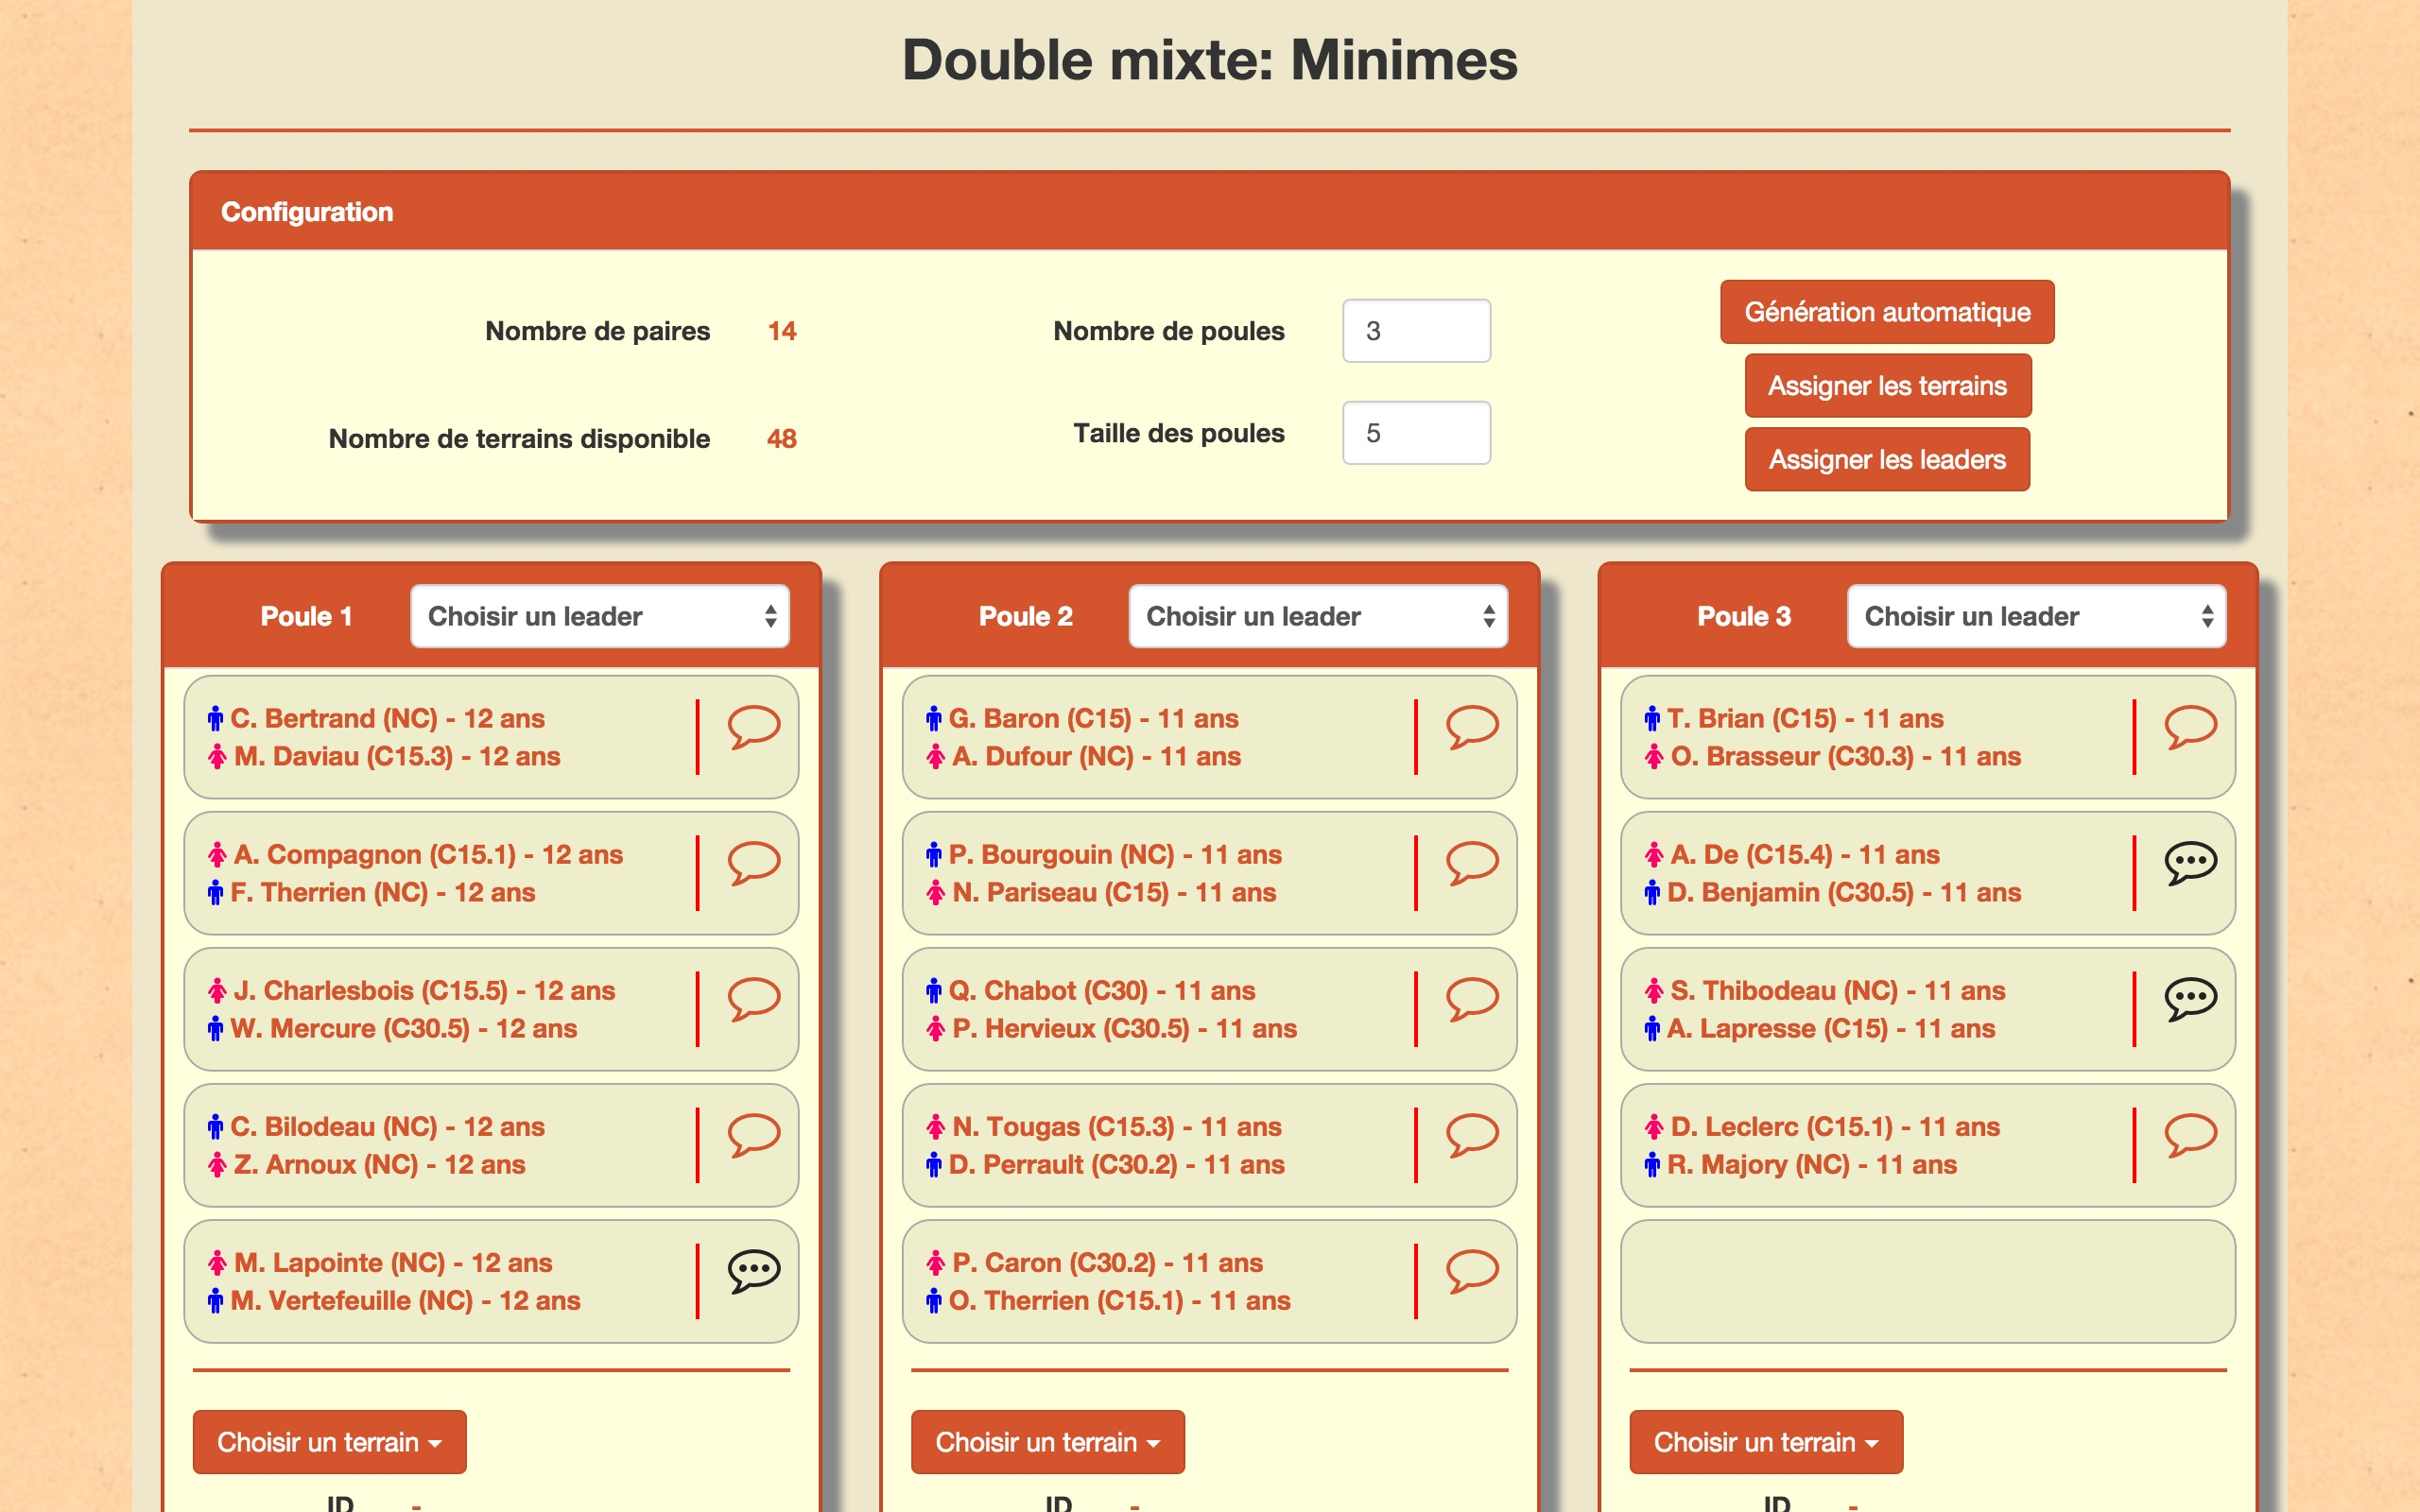
\includegraphics[scale=0.15]{creation-poules/creation-poules.jpg}
\caption{Page de création des poules}
\end{figure}

Le module de configuration des poules permet de connaître le nombre de paires et de terrain disponibles, de définir le nombre et la taille des poules du tournoi, et d'interagir automatiquement avec ces poules à l'aide de 3 boutons d'assistance à la création des poules.

\begin{figure}[H]
\centering
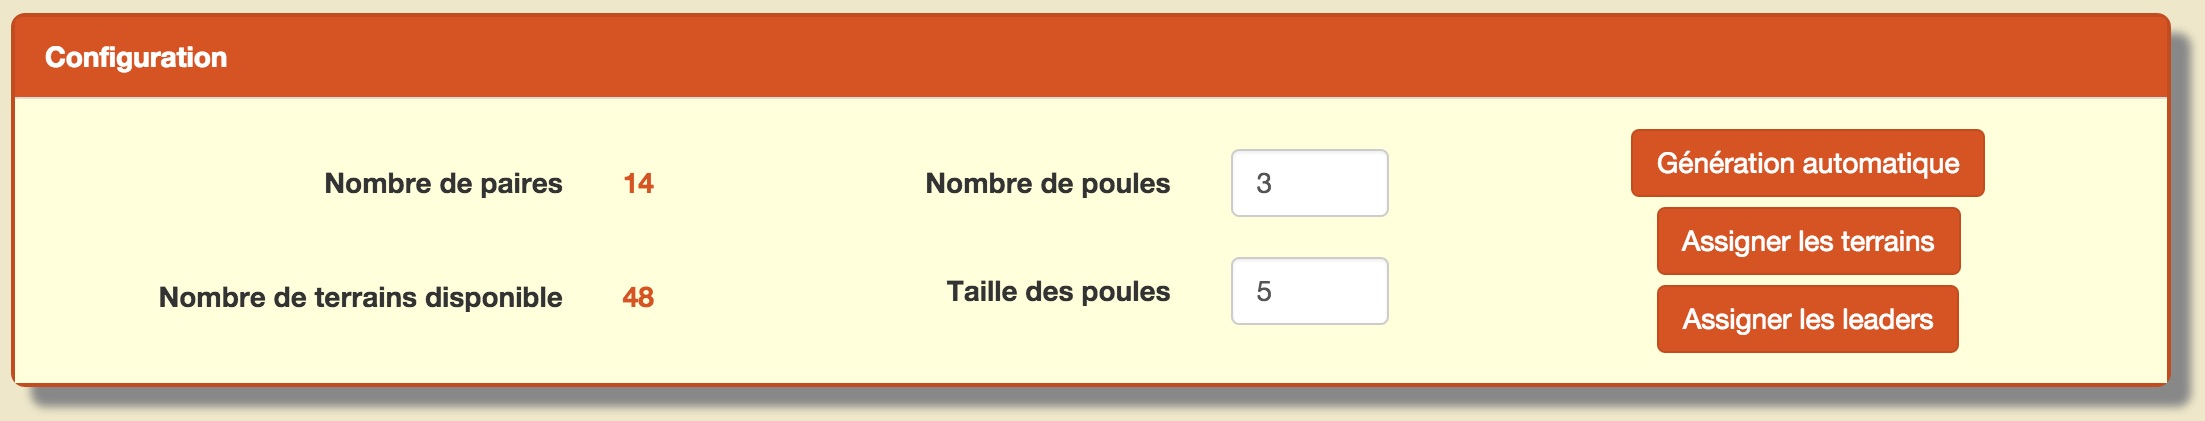
\includegraphics[scale=0.15]{creation-poules/creation-poules-configuration.jpg}
\caption{Module de configuration de création des poules}
\end{figure}

En modifiant la taille des poules (\textit{respectivement}, le nombre de poules), le nombre de poules (\textit{respect.}, la taille des poules) s'adaptent automatiquement pour permettre à toutes les paires d'être dans une poule.\newline

Les boutons d'assistance à la création des poules sont les suivants:

\begin{itemize}
\item \textit{Génération automatique} : ce bouton permet d'assigner automatiquement les paires par poules, les leaders, et les terrains de chacunes des poules ;
\item \textit{Assigner les terrains} : ce bouton permet d'assigner automatiquement les terrains de toutes les poules ;
\item \textit{Assigner les leaders} : ce bouton permet d'assigner automatiquement les leaders de toutes les poules
\end{itemize}
\bigskip

Les poules peuvent, à tout moment, être éditées. Un leader peut être assigné à une poule, en sélectionnant un joueur parmi tous les joueurs de la poule. Pour ce faire, sélectionnez un joueur dans la liste déroulante en titre du module de la poule.

\begin{figure}[H]
\centering
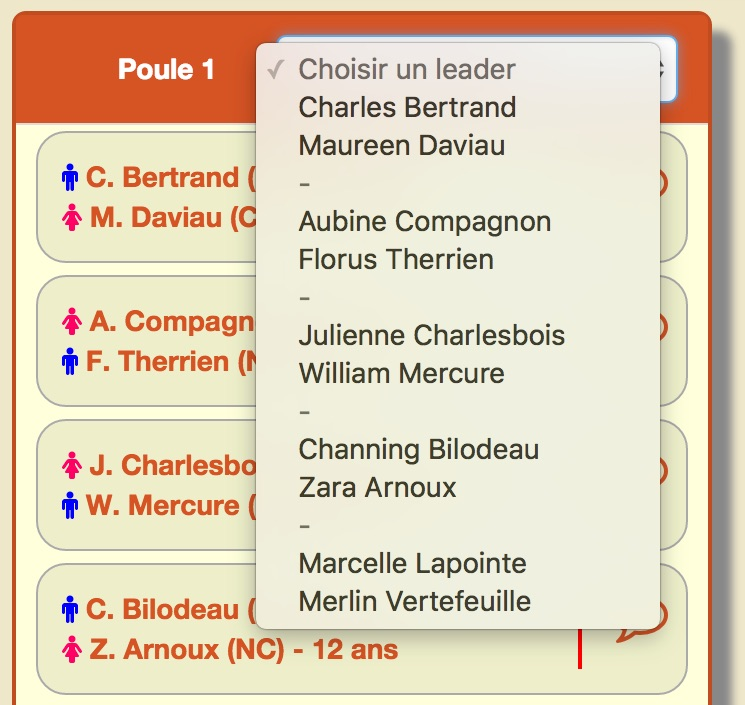
\includegraphics[scale=0.35]{creation-poules/creation-poules-leader.jpg}
\caption{Sélection du leader d'une poule}
\end{figure}

Le procédé pour assigner manuellement un terrain à une poule est similaire à celui de l'assignation d'un leader, sauf que cette sélection se trouve en bas du module de la poule. En cliquant sur le bouton \textit{Choisir un terrain}, une liste déroulante propose tous les terrains disponibles.

\begin{figure}[H]
\centering
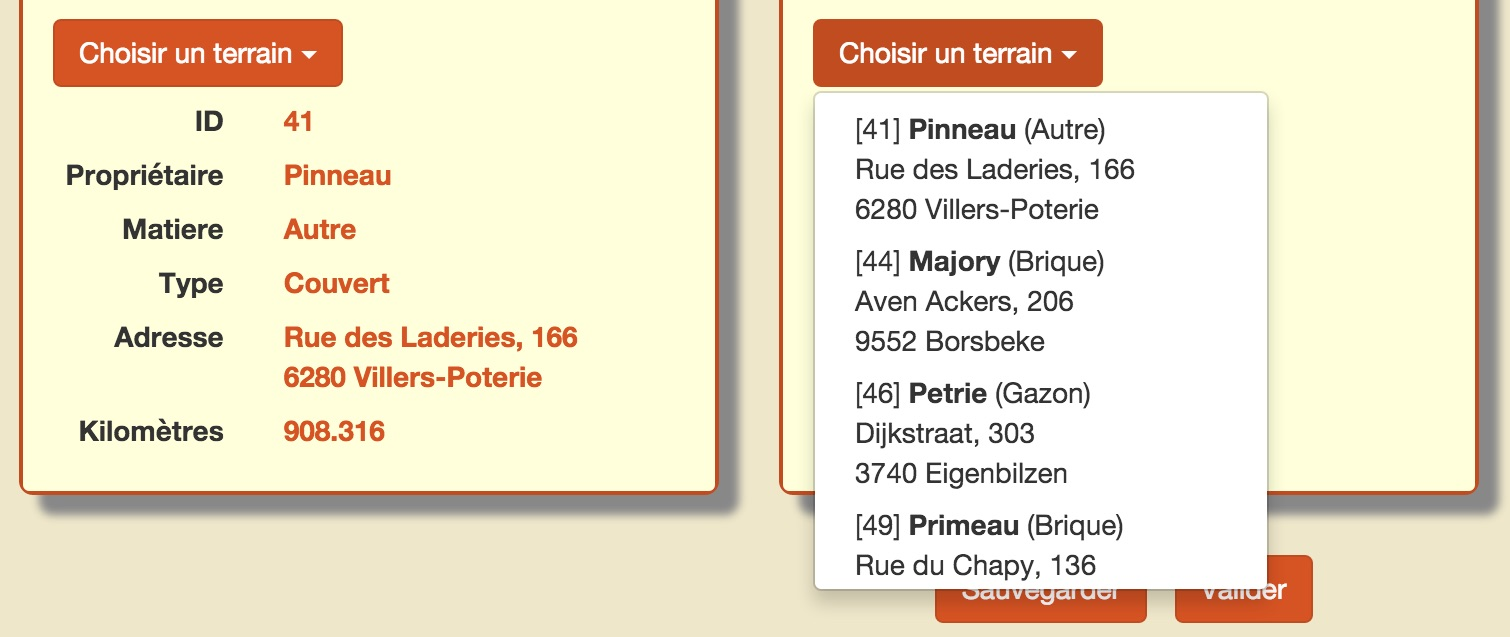
\includegraphics[scale=0.2]{creation-poules/creation-poules-terrain.jpg}
\caption{Sélection d'un terrain d'une poule}
\end{figure}

Dès que le terrain a été sélectionné, les informations du terrain sont résumées, tout en indiquant le nombre de kilomètres total que les joueurs de la poule doivent parcourir au minimum. Si le terrain est déjà en cours d'utilisation dans ce tournoi ou dans un autre tournoi, un petit avertissement en rouge le signale. En cliquant sur ce bouton, vous pouvez savoir rapidement dans quel tounoi ce terrain est déjà utilisé.

\begin{figure}[H]
\centering
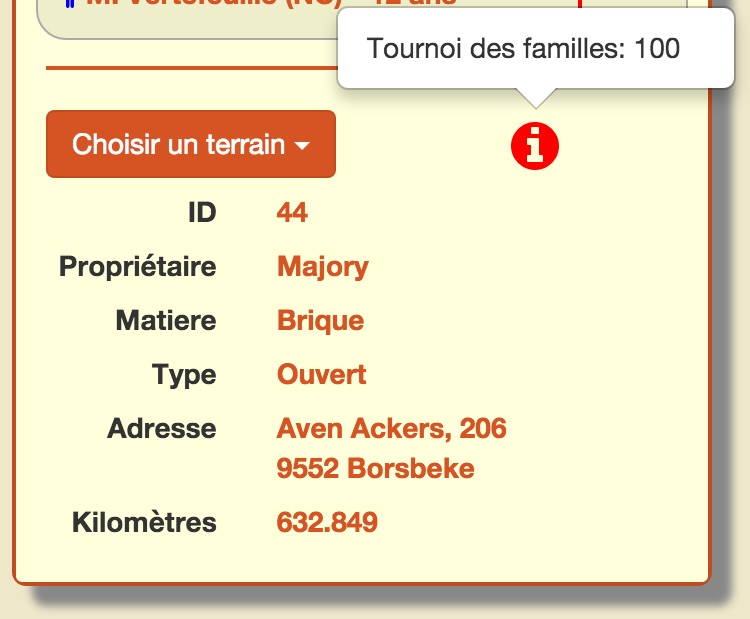
\includegraphics[scale=0.4]{creation-poules/creation-poules-avertissement.jpg}
\caption{Avertissement d'un terrain déjà utilisé}
\end{figure}

L'information sur le kilométrage total permet d'estimer l'empreinte carbone de la poule, qui peut être un paramètre que le responsable du tournoi pourrait souhaiter minimiser. Les boutons d'assignation automatique tentent de minimiser cette valeur pour toutes les poules, tout en choisissant comme leader le joueur le plus proche du QG de ASMAE.\newline

Les paires peuvent être manuellement permutées, au sein d'une poule ou entre deux poules différentes, en utilisant deux interactions possibles :

\begin{itemize}
\item la première interaction consiste à faire un \textbf{\textit{drag-and-drop}} d'une case d'une paire vers une autre case d'une autre paire. Cette interaction a l'avantage d'être intuitive.
\item la deuxième interaction consiste à faire un \textbf{\textit{click-and-switch}} d'une case d'une paire vers une autre case d'une autre paire. Cette interaction a l'avantage d'être facilement réalisable, même avec un nombre et des tailles de poules importants.
\end{itemize}

\begin{figure}[H]
\centering
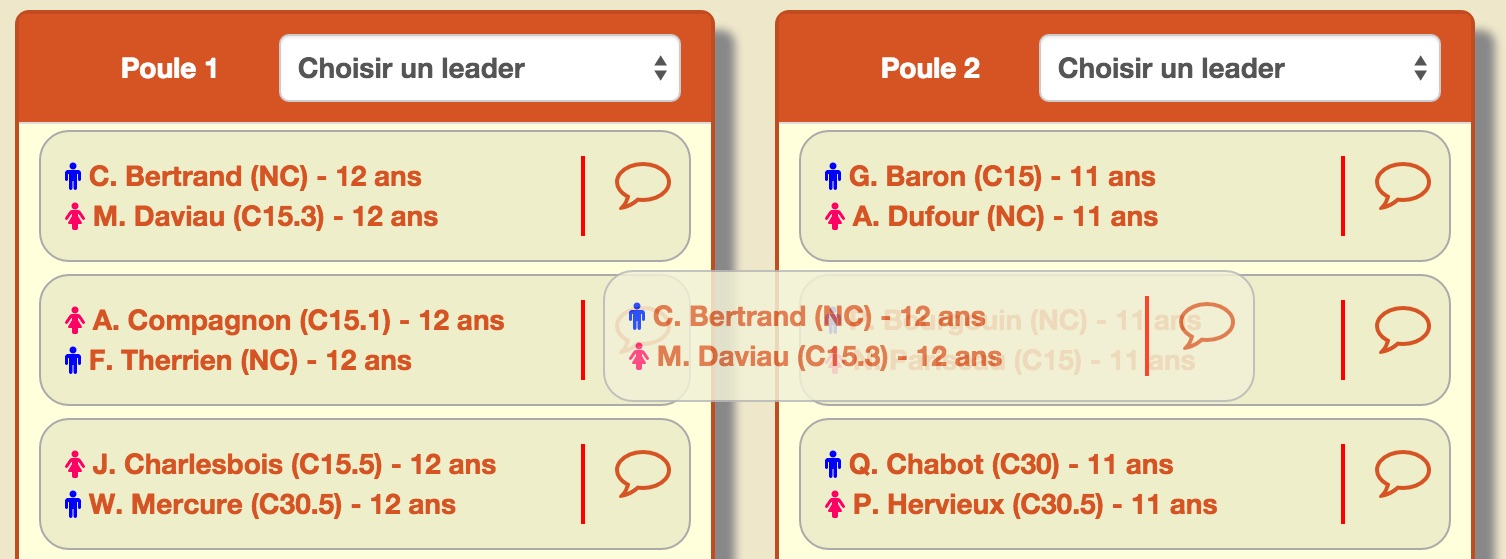
\includegraphics[scale=0.25]{creation-poules/creation-poules-dragndrop.jpg}
\caption{Interaction \textit{drag-and-drop} pour permuter deux paires}
\end{figure}

Il est aussi possible de créer les poules en prenant en compte les remarques et souhaits des paires. Chaque paire possède une icône de \textit{bulle de dialogue} à sa droite. Les bulles vides indiquent que la paire n'a aucune remarque ou souhait, tandis que les bulles avec trois points sont des paires ayant des commentaires. En passant le curseur sur une bulle remplie, les commentaires de la paire s'affichent à l'écran.

\begin{figure}[H]
\centering
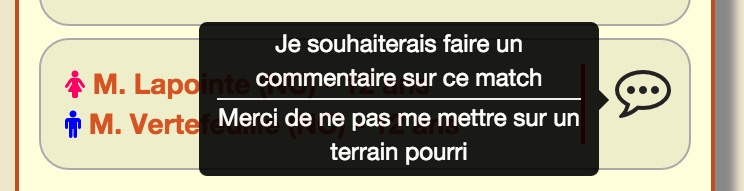
\includegraphics[scale=0.45]{creation-poules/creation-poules-commentaire.jpg}
\caption{Commentaire d'une paire}
\end{figure}

Si l'on souhaite enregistrer l'état actuel de la création des poules, on peut cliquer sur le bouton \textit{Sauvegarder} en bas de la page. Dès que toutes les poules ont des leaders et des terrains assignés, il est possible de finaliser la création des poules, en cliquant sur le bouton \textit{Valider}. Si des terrains ont des avertissements, une boîte de dialogue demande clairement à l'utilisateur de confirmer la validation des poules, malgré les conflits sur ces terrains.

\subsubsection{Gestion des poules}

La deuxième page des poules d'un tournoi est la gestion des poules. Elle est accessible à partir de la page \enquote{Gestionnaire des tournois}, en cliquant sur le bouton du tournoi qui se trouve à la colonne \textit{Scores}.

\begin{figure}[H]
\centering
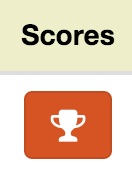
\includegraphics[scale=0.45]{gestion-poules/gestion-poules-bouton.jpg}
\caption{Bouton d'accès à la gestion des poules}
\end{figure}

Ce bouton est cliquable uniquement lorsque le status du tournoi est :

\begin{itemize}
\item \textbf{Poules validées} : c'est le status du tournoi lorsque les poules ont été totalement créées et validéés, prêtes pour imprimer les \textit{score boards} et pour encoder les scores.
\item \textbf{Poules terminées} : c'est le status du tournoi lorsque toutes les poules ont été encodées, et donc la création de l'arbre d'élimination peut commencer
\end{itemize}
\bigskip

La page de gestion des poules se présente avec un module par poule.

\begin{figure}[H]
\centering
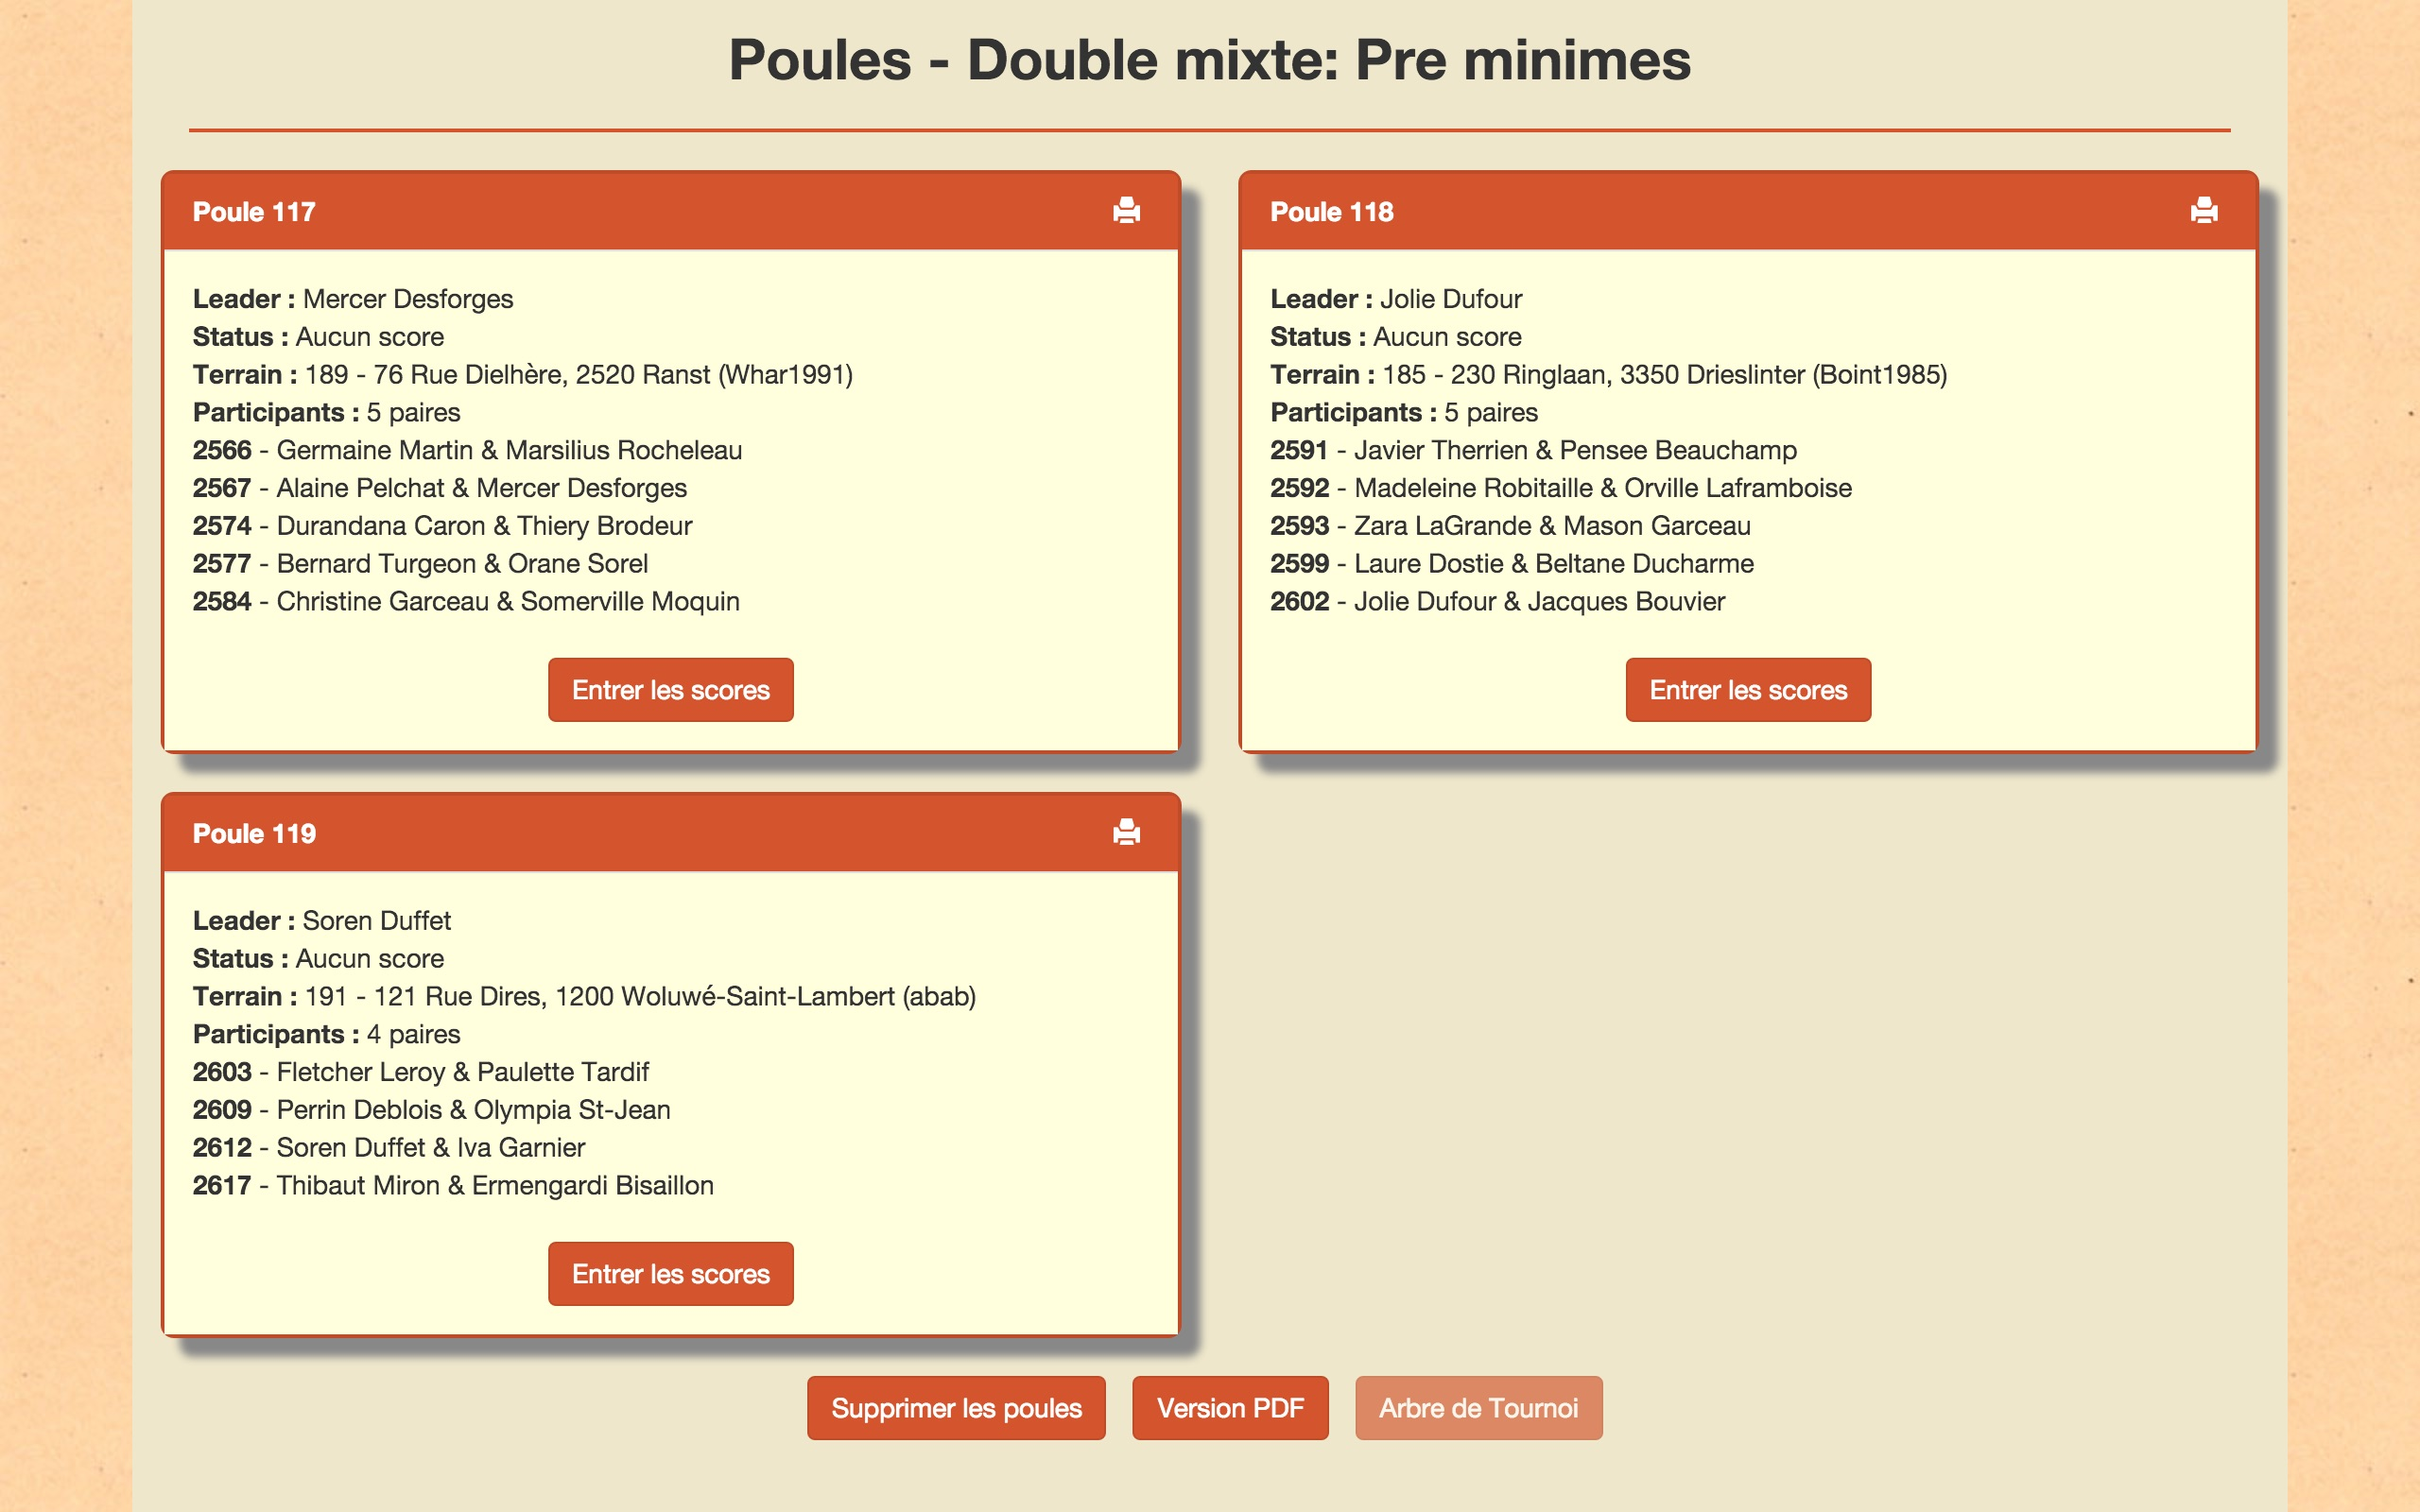
\includegraphics[scale=0.15]{gestion-poules/gestion-poules.jpg}
\caption{Page de gestion des poules d'un tournoi}
\end{figure}

Chaque poule contient le nombre de paires, la liste de toutes les paires, le leader, et le terrain assigné. Il est possible d'obtenir le \textit{scoreboard} de la poule, en cliquant sur bouton dans le coin droit supérieur du module, avec une icône d'imprimante.

\begin{figure}[H]
\centering
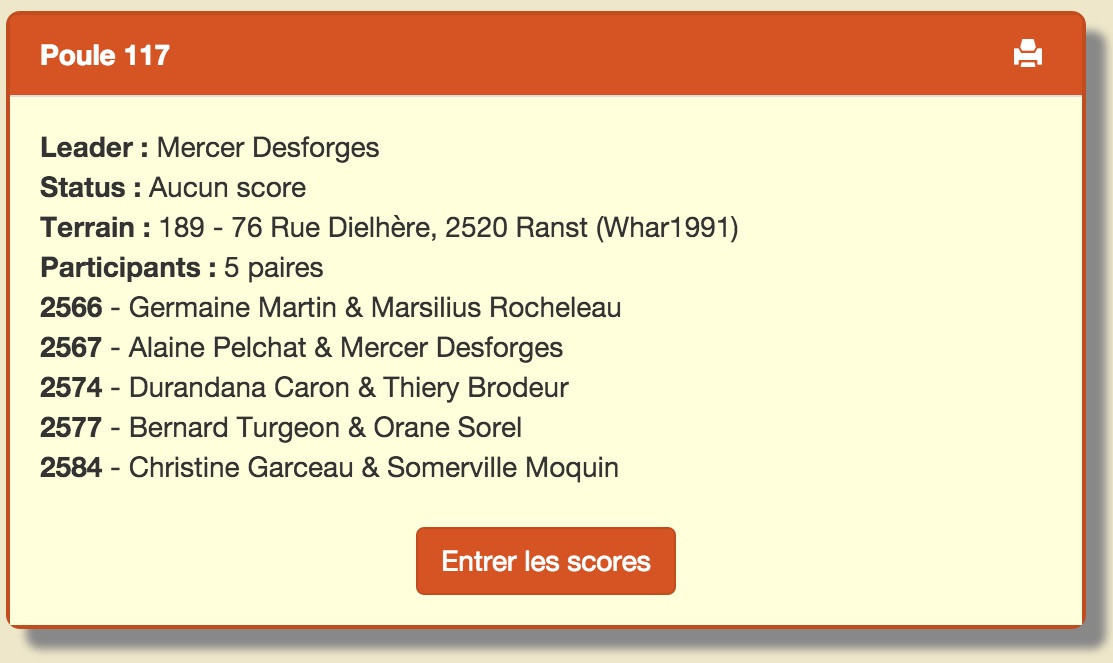
\includegraphics[scale=0.3]{gestion-poules/gestion-poules-poule.jpg}
\caption{Module d'une poule de la page de gestion des poules}
\end{figure}

Il est possible d'encoder les scores des matchs de la poules en cliquant sur le bouton \textit{Entrer les scores}. Ce bouton permet d'accéder à un \textit{score board} interactif. Les scores doivent être entrés dans les champs, où le premier champ de la case est le nombre de points de la paire sur la ligne, et le deuxième champ est le nombre de points de la paire sur la colonne. Les scores sont symétriques par rapport à la diagonale : par exemple, le score à la première ligne et deuxième colonne est à tout moment l'inverse du score à la deuxième ligne et première colonne du \textit{score board}.

\begin{figure}[H]
\centering
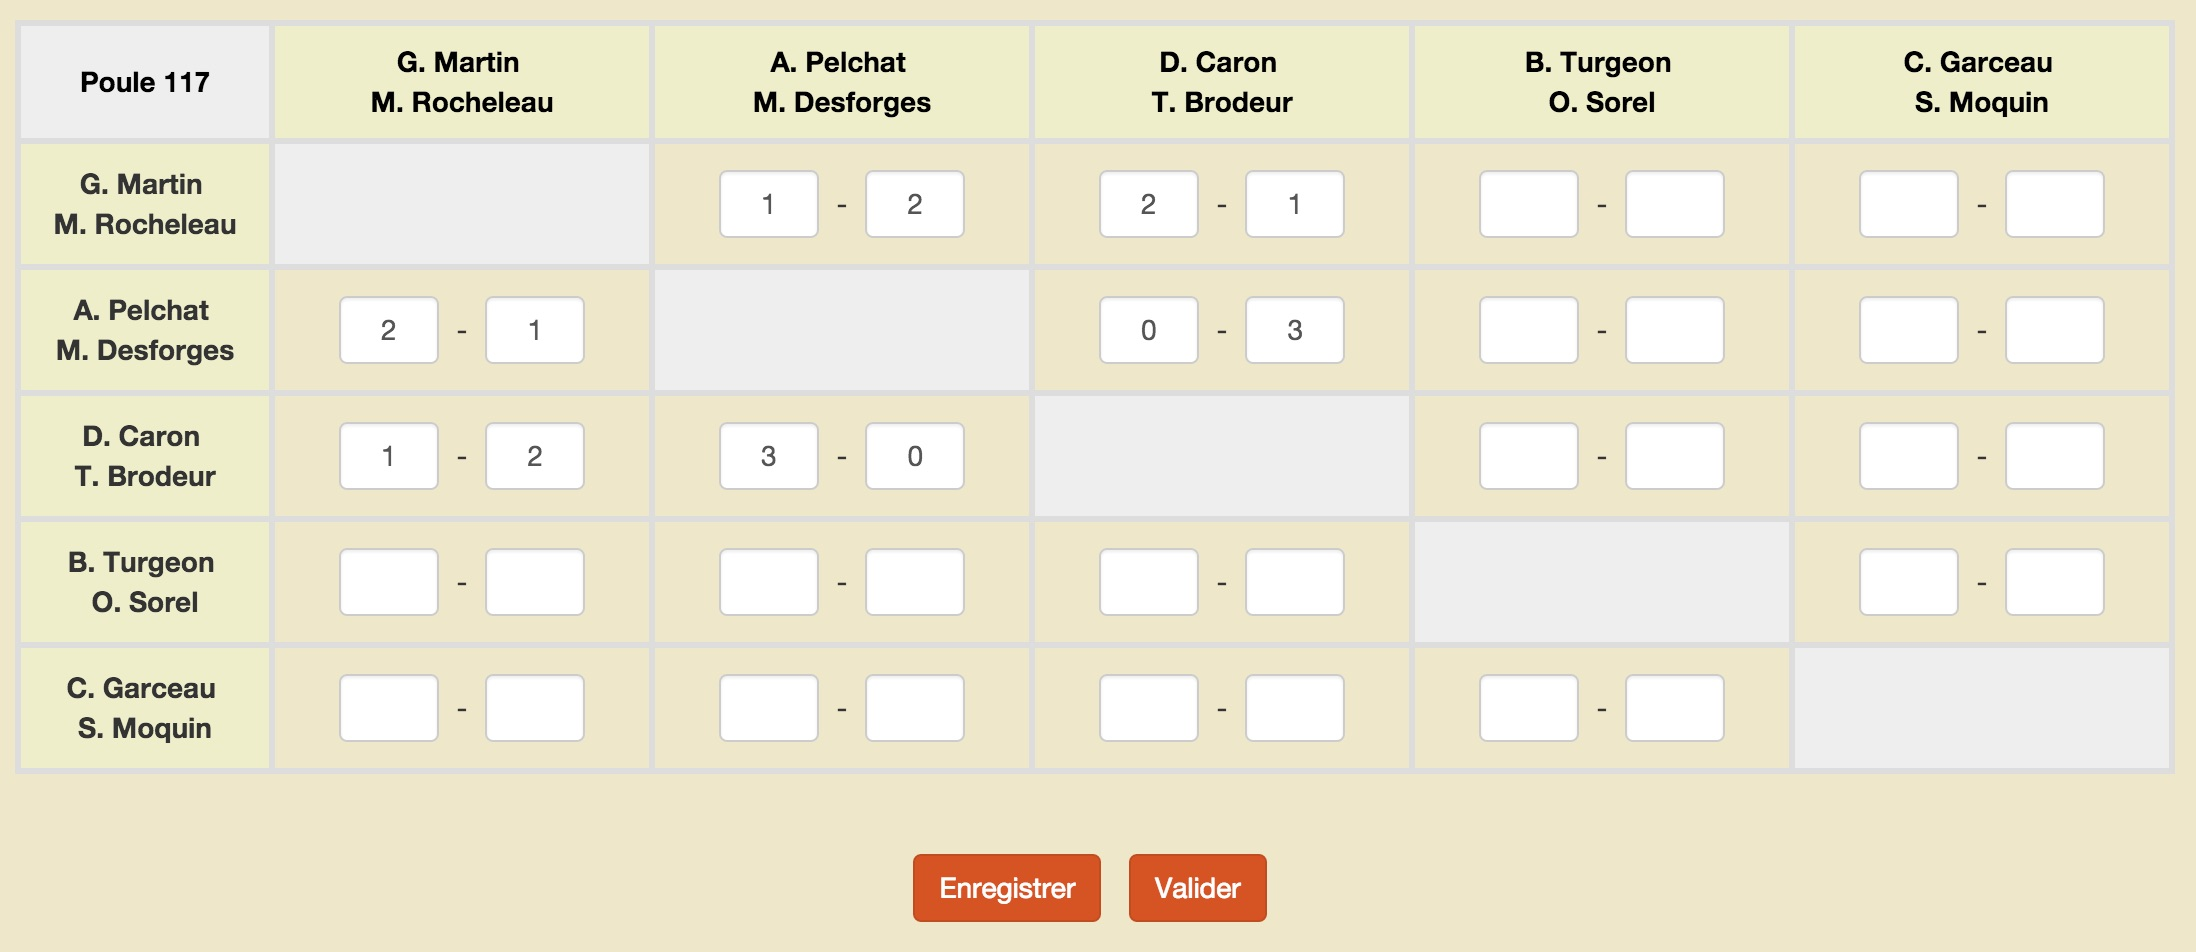
\includegraphics[scale=0.15]{gestion-poules/gestion-poules-score.jpg}
\caption{Page du \textit{score board} interactif de la poule}
\end{figure}

Le \textit{score board} interactif peut être enregistré, ou validé pour afficher définitivement les scores de la poule. Lorsque les scores sont validés, les scores totaux des paires de la poule sont résumés sur la page de gestion des poules.

\begin{figure}[H]
\centering
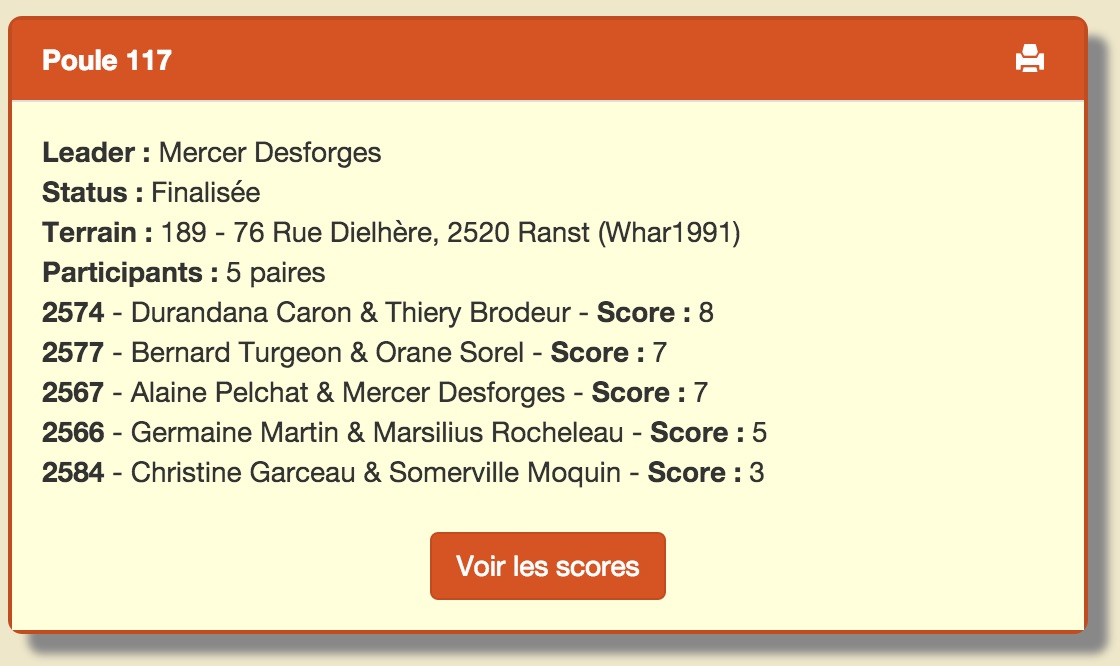
\includegraphics[scale=0.3]{gestion-poules/gestion-poules-encode.jpg}
\caption{Module d'une poule encodée dans la page de gestion des poules du tournoi}
\end{figure}

En bas de la page de la gestion des poules, il est possible de télécharger les \textit{score boards} de toutes les poules à la fois en cliquant sur le bouton \textit{Version PDF}. Il est également possible de supprimer toutes les poules, et revenir à l'étape de \enquote{Poules sauvegardées} du tournoi, en cliquant sur le bouton \textit{Supprimer les poules}. Enfin, le bouton \textit{Arbre de Tournoi} permet d'accéder à la page de l'arbre d'élimination, uniquement accessible lorsque toutes les poules ont été encodées.

\subsection{L'arbre d'élimination}

Toutes les fonctionnalités des tournois propres aux arbres sont accessibles uniquement aux tournois dont le status sont l'un des deux suivants :

\begin{itemize}
\item \textbf{Poules terminées} : lorsque toutes les poules ont été encodées, et que l'arbre d'élimination n'a pas été créé ou est non terminé (\textit{c'est-à-dire} qu'il n'y a pas encore de gagnant) ;
\item \textbf{Tournoi terminé} : lorsque l'arbre d'élimination a été complètement encodé, et qu'il y a un gagnant du tournoi
\end{itemize}
\bigskip

Il n'y a qu'une seule page spécifique à l'arbre d'élimination du tournoi, qui s'adapte automatiquement aux 2 cas suivants :

\begin{itemize}
\item \textbf{Création de l'arbre} : toutes les poules ont étés encodées, et aucun arbre d'élimination n'a été créé
\item \textbf{Gestion de l'arbre} : Toutes les poules ont été encodées, et un arbre d'élimination a été créé et enregistré
\end{itemize}
\bigskip

Cette page est accessible de deux manières différentes, qui sont complètement symétriques :

\begin{itemize}
\item soit par la page principale de \enquote{Gestionnaire des poules}, en cliquant sur le bouton sous la colonne \textit{Arbre de tournoi}.
\item soit par la page de gestion des poules, lorsque toutes les poules ont été encodées, en cliquant sur le bouton \textit{Arbre du tournoi} en bas de la page.
\end{itemize}
\bigskip

\begin{figure}[H]
\centering
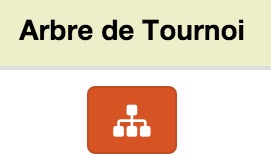
\includegraphics[scale=0.45]{creation-arbre/creation-arbre-bouton.jpg}
\caption{Accés à la page de l'arbre, depuis la page de gestion des tournois}
\end{figure}

\subsubsection{Création de l'arbre}

Si aucun arbre d'élimination n'a été préalablement enregistré, ou bien que toutes les poules ont été récemment encodées, alors les deux accès à la page de l'arbre d'élimination sont accessibles. En accédant à la page de l'arbre du tournoi, puisqu'aucun arbre n'a encore été créé, il est demandé à l'utilisateur de choisir les paires à sélectionner pour le tournoi d'élimination.

\begin{figure}[H]
\centering
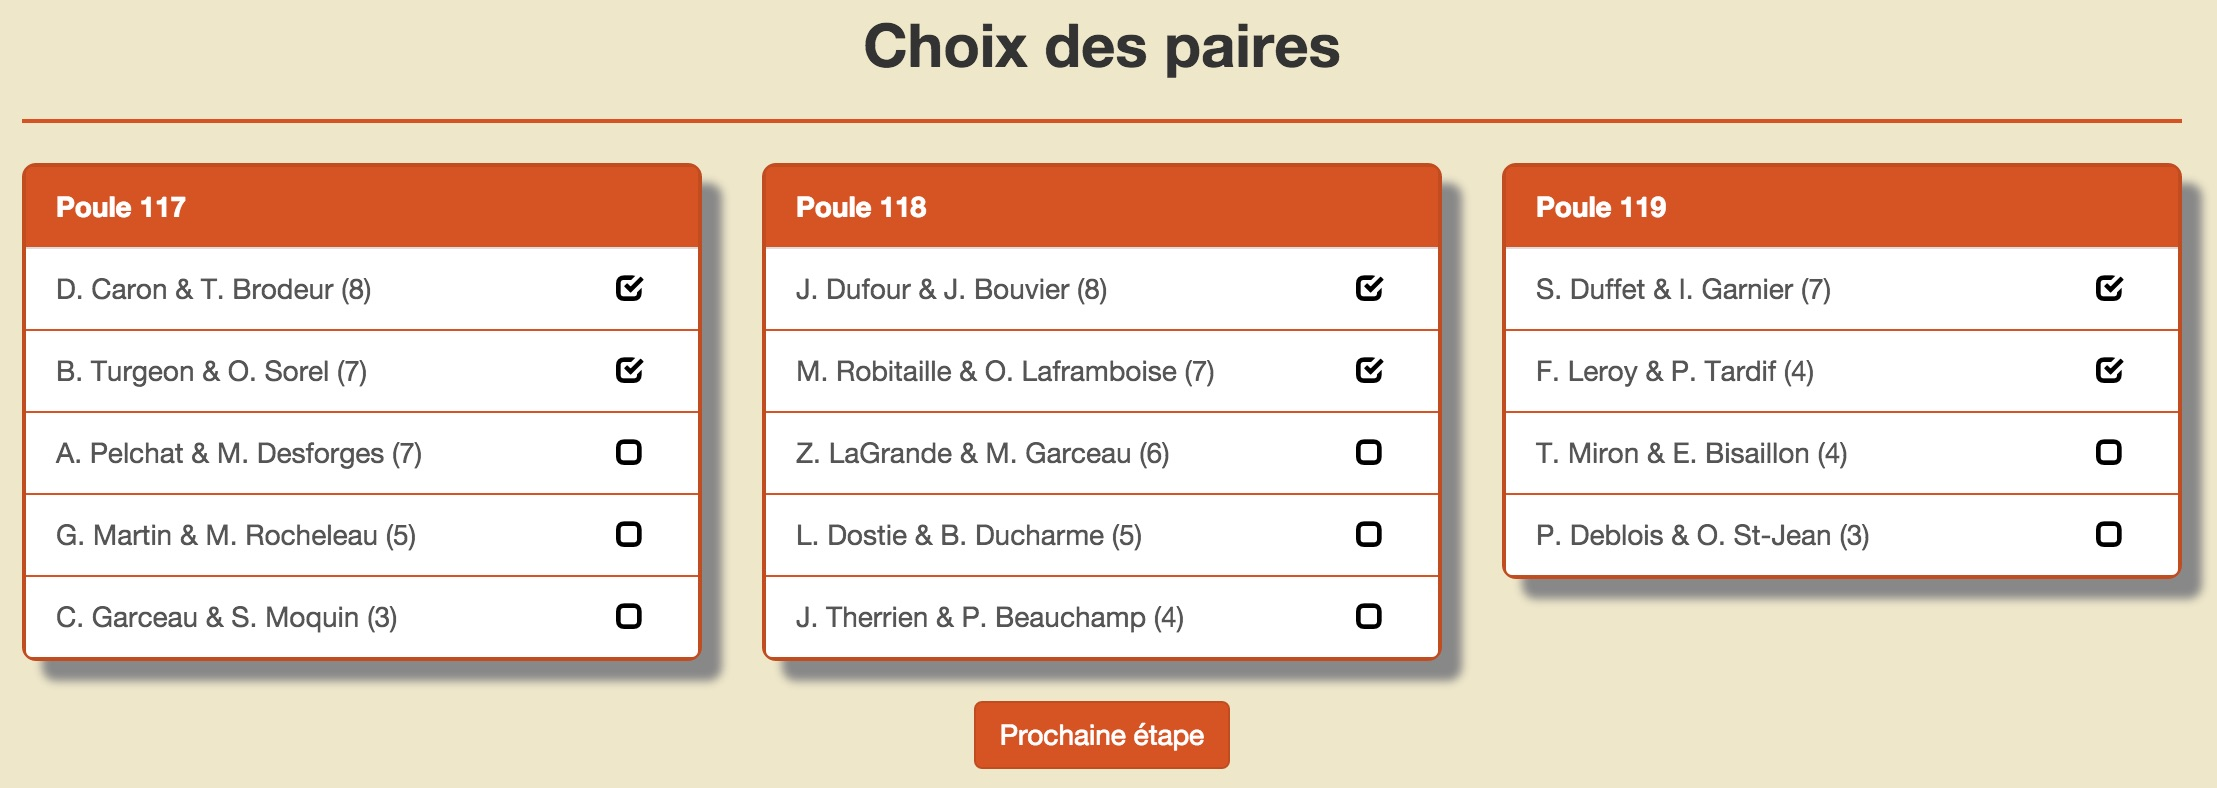
\includegraphics[scale=0.15]{creation-arbre/creation-arbre-etape1.jpg}
\caption{Première étape de la création d'un arbre - sélection des paires}
\end{figure}

Les paires sont triées par leurs points totaux au sein d'une poule, de la paire aux points les plus élevés jusqu'à la paire aux points les moins élevés. Les scores sont affichés entre parenthèses à côté des noms des joueurs de la paire. L'icône à droite de la case d'une paire indique si la paire est sélectionnée ou non pour l'arbre d'élimination. Pour modifier l'état de la sélection de la paire, il faut cliquer sur la case de la paire.\newline

Dès que les paires cochées sont celles que l'on souhaite avoir pour commencer l'arbre d'élimination, on peut poursuivre le processus de création de l'arbre d'élimination en cliquant sur le bouton \textit{Prochaine étape}, tout en bas de la page.\newline

Sur cette deuxième et dernière page de création de l'arbre, il est demandé de choisir un terrain et l'ordre des paires au départ de l'arbre. Ces deux paramètres sont divisés en deux modules différents :

\begin{itemize}
\item Le module \enquote{Terrain}, en haut, permet d'assigner un terrain de la même manière que lors de la création des poules : soit manuellement en cliquant sur le bouton \textit{Choisir un terrain}, soit automatiquement en cliquant sur le bouton \textit{Assigner Terrain} ;
\item Le module \enquote{Premier Round}, en bas, permet d'ordonner les paires au début de l'arbre d'élimination via l'interaction \textbf{\textit{drag-and-drop}}
\end{itemize}
\bigskip

Pour ordonner efficacement les paires au départ de l'arbre d'élimination, l'identifiant de la poule et la position dans la poule (ordonné selon le score total) est précisé pour chacune des paires.

\begin{figure}[H]
\centering
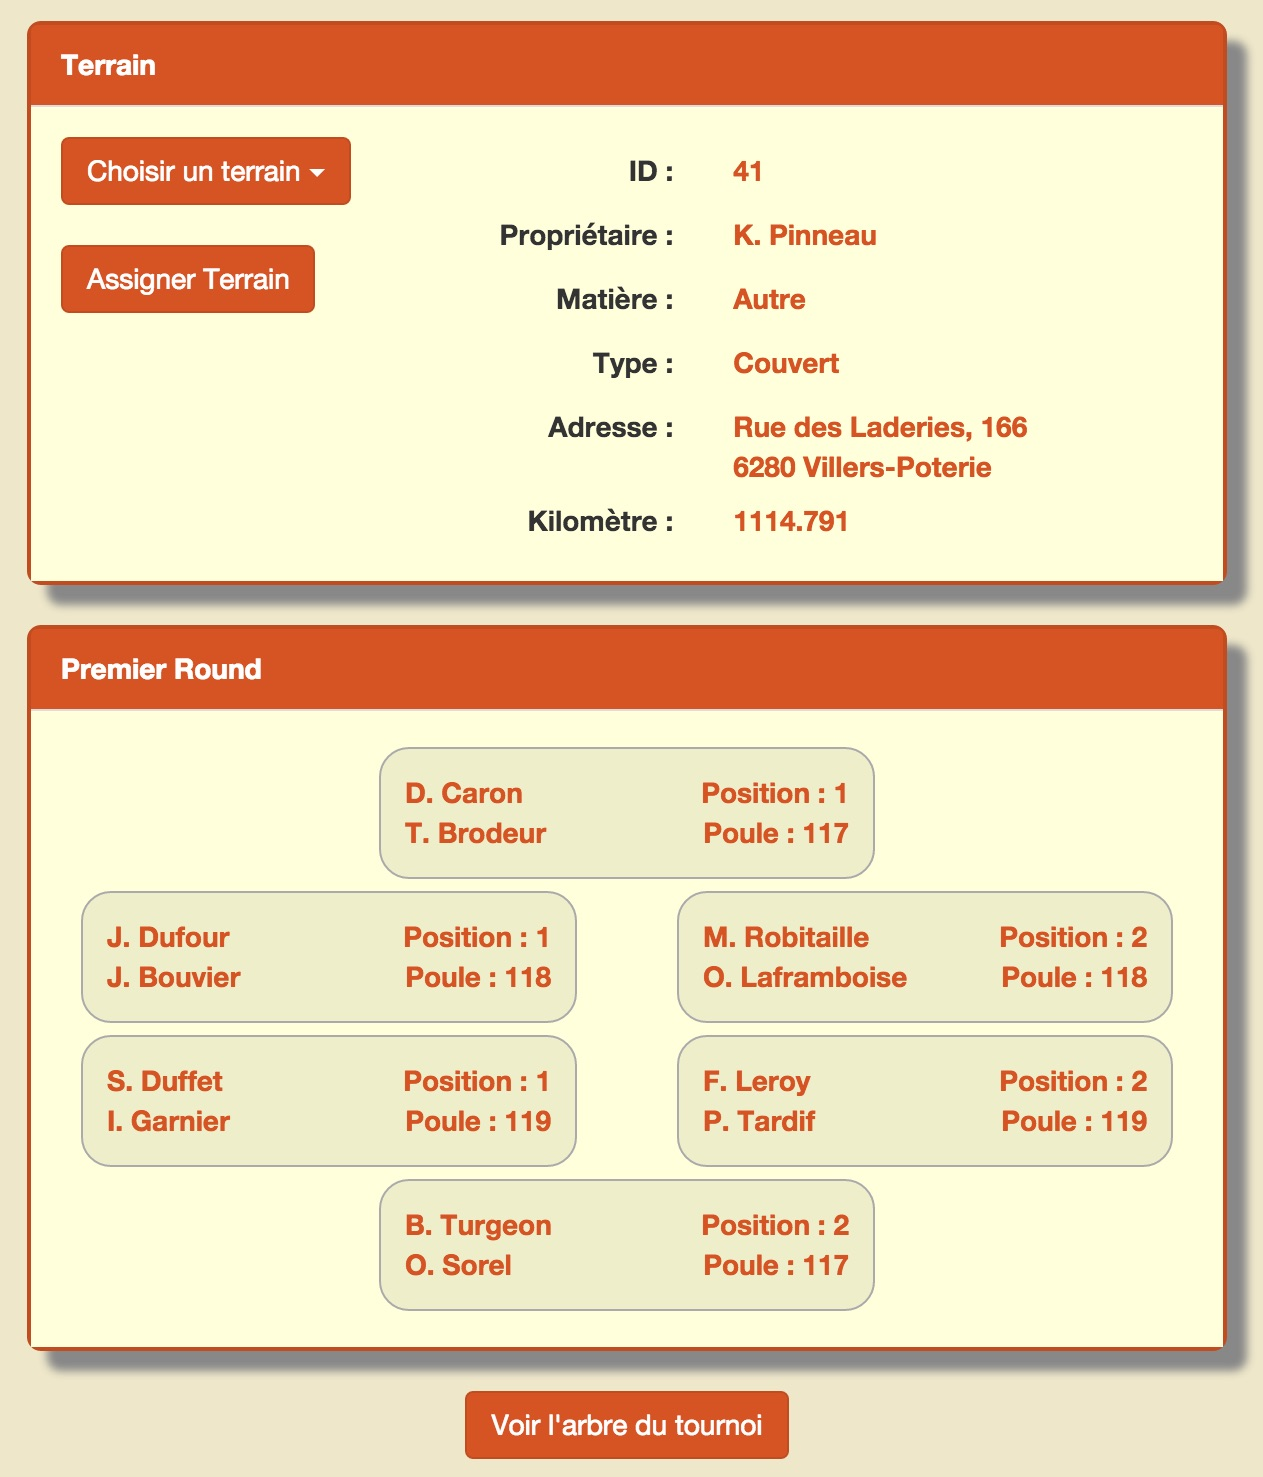
\includegraphics[scale=0.3]{creation-arbre/creation-arbre-etape2.jpg}
\caption{Deuxième étape de la création de l'arbre - sélection du terrain et de l'ordre des paires}
\end{figure}

Pour finaliser le processus de création de l'arbre, il suffit de cliquer sur le bouton \textit{Voir l'arbre du tournoi}, en bas de la page. N'oubliez pas d'enregistrer l'arbre dès qu'il a été créé, sinon vous devez recommencer le processus de création de l'arbre depuis le début ! Pour enregistrer l'arbre créé, cliquez simplement sur le bouton \textit{Enregistrer} en bas de la page de gestion de l'arbre d'élimination


\subsubsection{Gestion de l'arbre}

Si un arbre d'élimination a été enregistré, alors la page de l'arbre d'élimination du tournoi permettra d'accéder directement à la page avec l'arbre interactif du tournoi.

\begin{figure}[H]
\centering
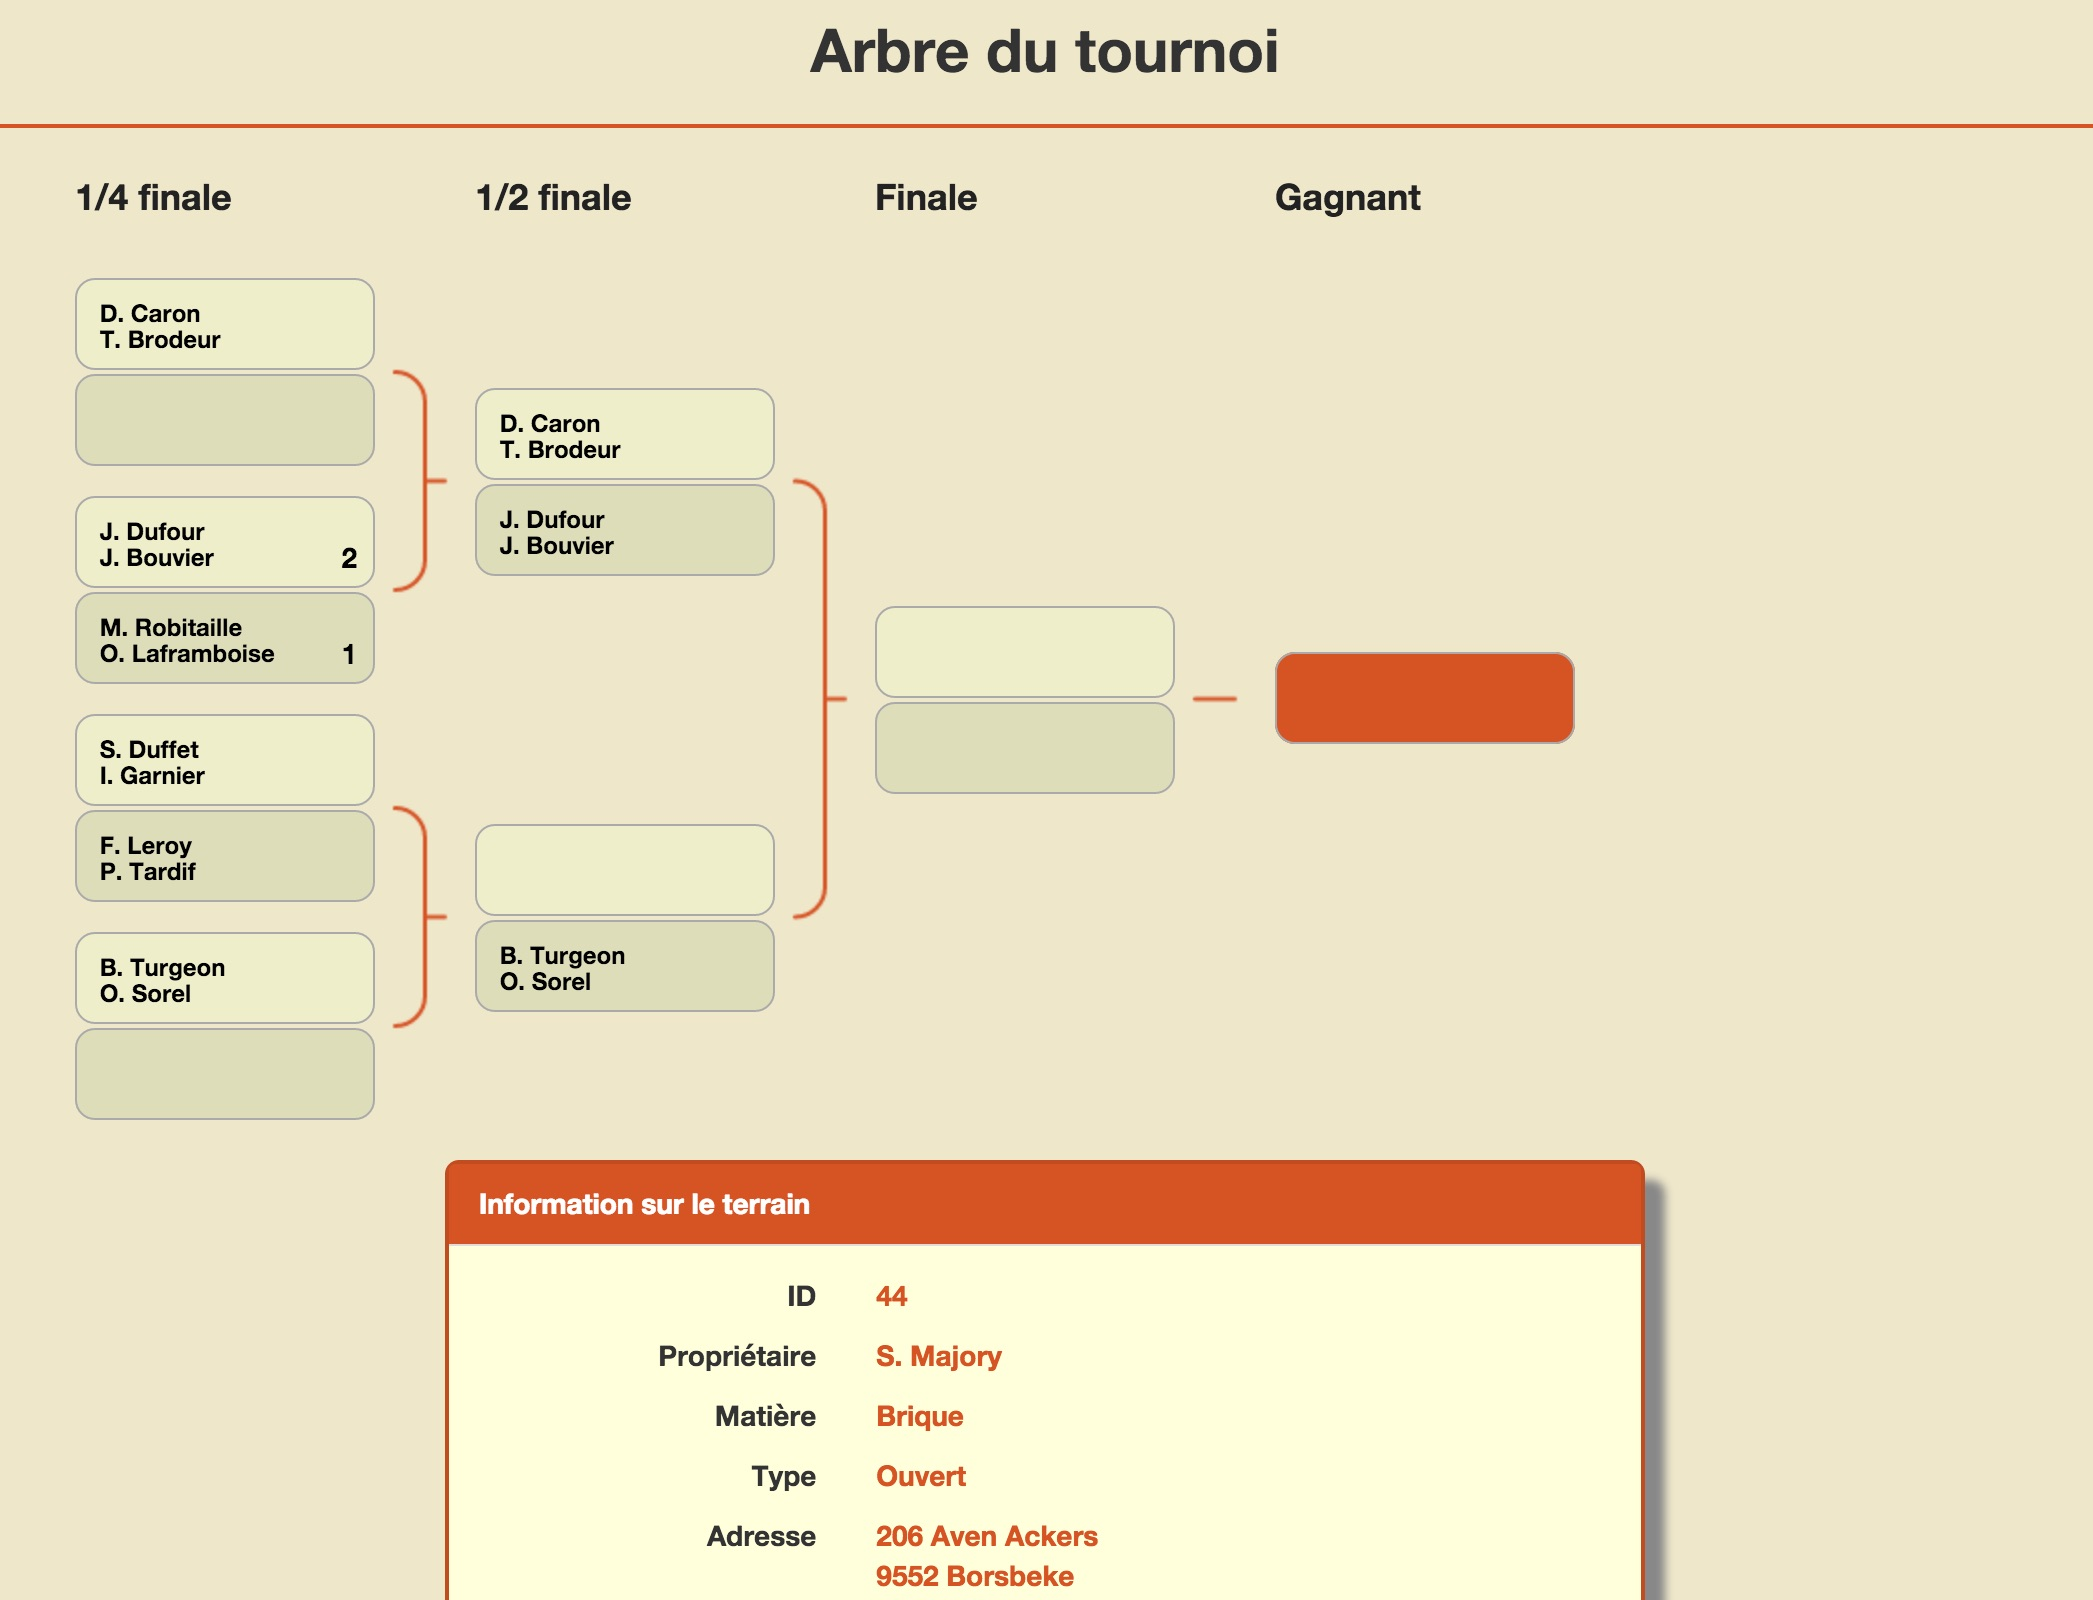
\includegraphics[scale=0.15]{gestion-arbre/gestion-arbre.jpg}
\caption{Page de gestion de l'arbre d'élimination}
\end{figure}

Cette page est divisée en deux parties :

\begin{itemize}
\item \textit{la partie du haut} contient un module interactif d'encodage de l'arbre d'élimination ;
\item \textit{la partie du bas} contient un module d'information sur le terrain du tournoi d'élimination, avec les boutons de gestion de l'arbre tout en bas de la page
\end{itemize}
\bigskip

L'arbre d'élimination donne une représentation de l'arbre du tournoi, où chaque case est une paire. Deux cases verticalement collées entre elles représentent le match des deux paires considérées, l'une contre l'autre.

\begin{figure}[H]
\centering
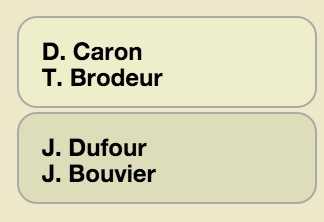
\includegraphics[scale=0.3]{gestion-arbre/gestion-arbre-match.jpg}
\caption{Match entre deux paires dans l'arbre d'élimination interactif}
\end{figure}

Pour encoder le score d'un match, il suffit de cliquer sur l'une des deux paires, et d'inscrire le score du match dans la boîte de dialogue. Ensuite, la paire gagnante sera automatiquement placée à l'étape suivante de l'arbre d'élimination. N'oubliez pas d'enregistrer l'arbre d'élimination après avoir encodé les scores, sinon l'arbre n'aura pas été mise à jour !\newline

Lorsque l'arbre d'élimination a complètement été encodé, c'est-à-dire lorsqu'il y a un gagnant dans le tournoi et que l'arbre a été enregistré, alors le status du tournoi devient \enquote{Tournoi terminé}.\newline

En plus du bouton \textit{Enregistrer}, qui permet d'enregistrer l'état de l'arbre d'élimination, deux autres boutons se trouve en bas de la page:

\begin{itemize}
\item \textit{Version PDF} permet d'imprimer l'arbre du tournoi et l'information du terrain ;
\item \textit{Enregistrer} permet d'enregistrer l'état de l'arbre du tournoi ;
\item \textit{Supprimer} permet de supprimer l'arbre d'élimination, et de revenir à l'étape de création de l'arbre d'élimination
\end{itemize}
\bigskip